\section{Data Analysis}
\label{section:Data:DataAnalysis}

For any kind of prediction model to work, the underlying dataset needs some kind of recognisable pattern for
the model to learn.
In order to analyse the predictebilty of the data we checked for white noise, and if the time-series followed a random walk.

\subsection*{Theory}

\begin{figure}[h!]
  \centering
  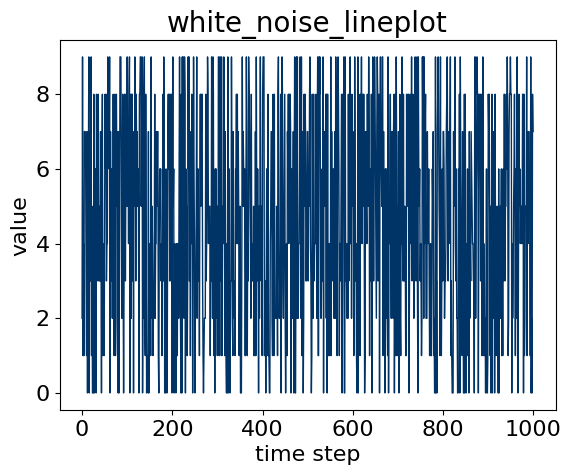
\includegraphics[width=\textwidth]{./figs/code_generated/data_exploration/white_noise_lineplot.png}
  \hfill
  \caption{A Random walk lineplot}
  \label{fig:dataset:white_noise}
\end{figure}
\begin{figure}[h!]
  \centering
  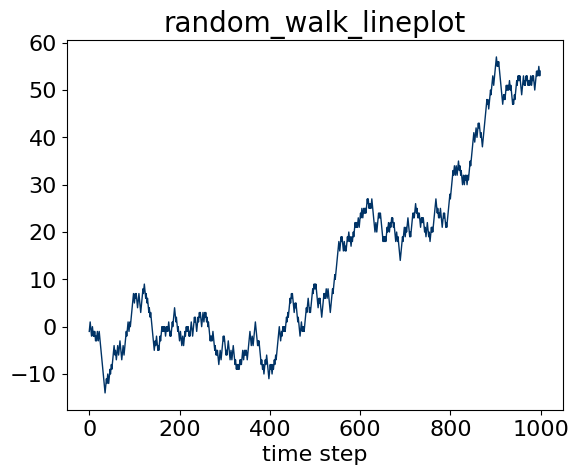
\includegraphics[width=\textwidth]{./figs/code_generated/data_exploration/random_walk_lineplot.png}
  \hfill
  \caption{A Random walk lineplot}
  \label{fig:dataset:random_walk}
\end{figure}

TODO [Move to B and T?]
White noise is just a random sample of numbers not following any pattern what so ever, as seen in
\Cref{fig:dataset:random_walk}.


A random walk is different from white noise, because the next value in the series is dependent on the previous value as seen in

\Cref{fig:dataset:random_walk}.

We chose a random sample of correlating categories to analyse,
and a set of highly seasonal categories.
Categories chosen was
%corr_categories cat: 2, 6, 9, 10, 11, 13, 20
%
%seasonal_categories_cat_name ["Vinterjakke",
%"Vintersko",
%"Langrennski",
%"Skisko",
%"Varmeovn",
%"Snøfreser",
%"Snøskuffe",]



By analysing a lag plot we can look for patterns in the data. A lag plot
show how much future values depend on past values.
TODO[Add lag plots].
The lag plot of.
% Write about dicky fuller test on dataset and decomposed resid.
% Write about how a lag plot of how a random walk looks like
% Write about how difference plot of random walk looks liks
% Write about lag plot and difference plot of our data 
% Check autocorrelation on random walk diff: https://machinelearningmastery.com/gentle-introduction-random-walk-times-series-forecasting-python/



